\chapter{The Tonnetz meets data}\label{ch:data}
The previous chapters treated the Tonnetz as a mathematical object. This chapter asks how real music moves on it.
We survey public datasets and software, describe a reproducible pipeline, and report a small four-corpus study.

\section{Public datasets}
\Cref{tab:datasets} lists open chord corpora suitable for Tonnetz analysis. They differ in three ways that matter:
\emph{representation} (chord labels such as Harte syntax \citep{harte2005}, Roman numerals, or full scores),
\emph{timing} (aligned to audio or to the score), and \emph{licence}.

\begin{table}[t]\centering\small
\begin{tabular}{@{}p{3.2cm}p{2.5cm}p{3.4cm}p{5.2cm}@{}}\toprule
Dataset & Size & Representation & Access\\\midrule
ChoCo \citep{deberardinis2023} & 18 integrated collections & JAMS; Harte, Roman, lead-sheet & \url{github.com/smashub/choco}, CC BY 4.0 (mostly)\\
Chordonomicon \citep{kantarelis2024} & $>$666\,000 songs & chord symbols + genre, year, sections & \url{github.com/spyroskantarelis/chordonomicon}; Hugging Face\\
ABC: Annotated Beethoven Corpus \citep{neuwirth2018} & 70 quartet movements & DCML harmony labels (TSV) & \url{github.com/DCMLab/ABC}, CC BY-NC-SA 4.0\\
Distant Listening Corpus \citep{hentschel2025} & 1\,326 pieces, 36 composers & DCML standard & \url{github.com/DCMLab/distant_listening_corpus}\\
NYU MARL annotations & 100 RWC-Pop + 195 USPop2002 songs & Harte-syntax \code{.lab} & \url{github.com/tmc323/Chord-Annotations}\\
music21 corpus \citep{cuthbert2010} & $\approx$400 Bach chorale files & full scores (MusicXML) & ships with \code{pip install music21}\\\bottomrule
\end{tabular}
\caption{Open corpora for Tonnetz studies. The last four rows are used in this chapter.}\label{tab:datasets}
\end{table}

\section{A reproducible pipeline}
\paragraph{Parsing.} Harte labels such as \code{A:min7/b3} or \code{C:(1,3,5,b7)} are parsed into pitch-class sets by
\code{harte\_to\_pcs}. DCML annotations list chord tones on the \emph{line of fifths} relative to the local tonic, so
a tone $k$ has pitch class $\text{tonic}+7k \bmod 12$; the local tonic is computed from the global key and the
Roman-numeral local key (\code{dcml\_chord\_pcs}). Bach chorales are ``chordified'' with music21 into vertical
slices.

\paragraph{Reduction to triads.} To place chords on the classical Tonnetz, each chord is reduced to its underlying
major or minor triad when it has one (\code{C:7}$\to$C, \code{A:min7}$\to$Am), following the ``majmin'' reduction
standard in chord-recognition evaluation \citep{raffel2014}. Diminished, augmented and suspended chords are dropped;
consecutive repeats are merged. For the Beethoven corpus we use the first three DCML chord tones (root, third,
fifth), so V$^7$ counts as V. For Bach we keep only slices whose pitch-class content is exactly a consonant triad.

\paragraph{Measurement.} For each pair of consecutive triads we record their distance in $\Gamma$ and their
voice-leading cost. As a \emph{null model} we shuffle the order of chords within each piece (keeping the piece's
chord vocabulary), merge any repeats created, and recompute the mean distance, averaged over 20 shuffles. A corpus
whose progressions are shorter than its own shuffles uses the Tonnetz ``locally'' beyond what its vocabulary alone
implies.

\section{Results}
\begin{table}[t]\centering\footnotesize\setlength{\tabcolsep}{4.5pt}
\begin{tabular}{@{}lrrcccccc@{}}\toprule
Corpus & Pieces & Transitions & Mean $d_\Gamma$ & Shuffled & $P(d{=}1)$ & $P(d{=}2)$ & $P(d{=}4)$ & Mean VL\\\midrule
Bach chorales & 400 & 13\,794 & 2.33 & 2.36 & 0.170 & 0.447 & 0.072 & 3.08\\
Beethoven (ABC) & 70 & 15\,097 & 2.39 & \textbf{2.58} & 0.131 & 0.469 & 0.075 & 3.05\\
RWC Pop & 100 & 11\,737 & 2.62 & \textbf{2.47} & 0.126 & 0.367 & 0.215 & 3.67\\
USPop2002 subset & 194 & 21\,945 & 2.49 & 2.44 & 0.154 & 0.415 & 0.197 & 3.57\\\midrule
Uniform random & -- & -- & 2.78 & -- & 0.130 & 0.261 & 0.217 & --\\\bottomrule
\end{tabular}
\caption{Consecutive-triad distances on the $PLR$ graph ($d_\Gamma$) and voice-leading cost (VL, semitones).
``Shuffled'' is the mean distance after randomly reordering each piece's chords. Produced by
\code{scripts/corpus\_analysis.py}.}\label{tab:corpus}
\end{table}

\begin{figure}[t]\centering
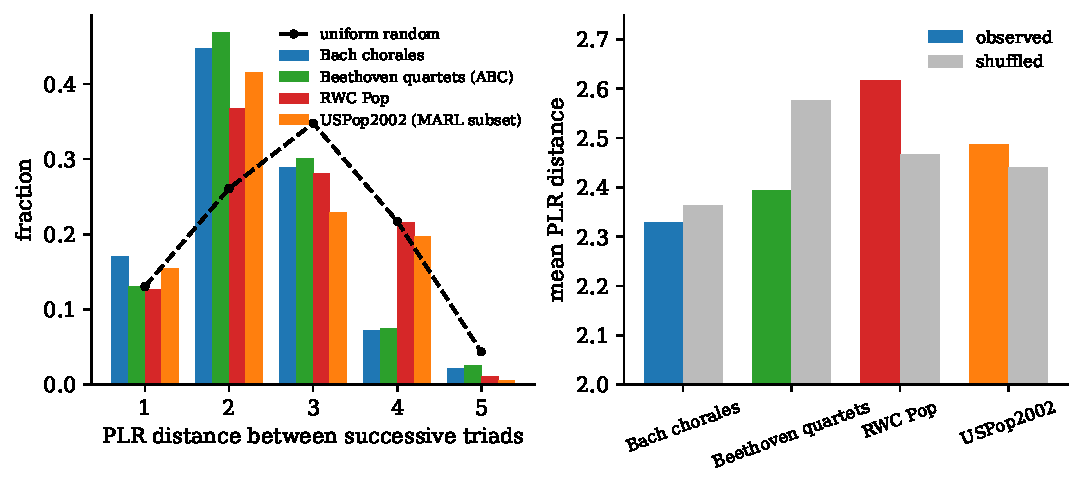
\includegraphics[width=\linewidth]{figures/corpus_plr.pdf}
\caption{Left: distribution of $PLR$ distances between successive triads, with the uniform baseline (dashed).
Right: observed mean distance versus the within-piece shuffle.}\label{fig:corpus}
\end{figure}

\Cref{tab:corpus} and \cref{fig:corpus} support four observations.
\begin{enumerate}
\item \emph{All four corpora are far more local than chance.} Distance 2 dominates everywhere. It is the distance
of motion by fifth (C$\to$G via Em, i.e.\ $L$ then $R$), the backbone of tonal harmony, and of motion by third
(C$\to$Am, C$\to$Em are distance 1).
\item \emph{Classical progressions exploit the Tonnetz beyond their vocabulary.} Beethoven's mean distance (2.39) is
well below that of his own shuffled chords (2.58); Bach's is slightly below (2.33 versus 2.36). The chorale
vocabulary is already so diatonic that shuffling it changes little.
\item \emph{Pop progressions do not.} Both pop corpora are \emph{longer} than their shuffles (RWC 2.62 versus
2.47). Almost the whole difference sits at distance 4, which occurs about three times as often in pop as in the
classical corpora.
\item \emph{Distance 4 in pop is the whole-step move.} Among distance-4 transitions, major-to-major root motion by
a whole step accounts for 77\% in USPop (45\% up, 32\% down) and 67\% in RWC. These are IV$\to$V, $\flat$VII$\to$I and
I$\to\flat$VII, idiomatic in rock \citep{biamonte2010,declercq2011}. In $\Gamma$ they cost four steps; in voice
leading they cost 6 semitones (all three voices move by a tone) against 3 for motion by fifth.
\end{enumerate}
The last point is a caution as much as a finding. The Tonnetz metric encodes a specific theory of closeness
(common tones and semitone voice leading). Pop's parallel whole-step motion is ``far'' under that theory but is not
perceived as a remote relation. Using the Tonnetz as a style descriptor, as in genre classification from Tonnetz
trajectories \citep{karystinaios2020}, measures distance from that theory, not a universal notion of harmonic
distance. Xu, Hall and Rohrmeier reach a related conclusion from pitch distributions: popular music shows higher
tonal focus but classical music more structured traversal of the Tonnetz \citep{xu2026}, building on the Tonal
Diffusion Model \citep{lieck2020}.

\paragraph{Limitations.} The reductions discard information (all seventh chords collapse to triads, and in Bach
non-triadic slices are skipped, which can create artificial jumps). The pop annotations are by trained students and
the classical ones by experts; annotation conventions differ. The corpora are small by modern standards; running
the same script on ChoCo or Chordonomicon would test whether the pattern generalises across genres and decades.

\section{From audio: the tonal centroid}
Harte, Sandler and Gasser \citep{harte2006} map a 12-bin chroma vector $c$ (energy per pitch class) to a point in
$\mathbb R^6$:
\[
\zeta(c)=\frac{1}{\|c\|_1}\sum_{\ell=0}^{11}c_\ell\,\Phi_\ell,\qquad
\Phi_\ell=\bigl(r_1\sin\tfrac{7\pi\ell}{6},\,r_1\cos\tfrac{7\pi\ell}{6},\,r_2\sin\tfrac{3\pi\ell}{2},\,r_2\cos\tfrac{3\pi\ell}{2},\,
r_3\sin\tfrac{2\pi\ell}{3},\,r_3\cos\tfrac{2\pi\ell}{3}\bigr),
\]
with $(r_1,r_2,r_3)=(1,1,\tfrac12)$. The three coordinate pairs place each pitch class on the circle of fifths, a
circle of minor thirds (4 points) and a circle of major thirds (3 points), which are exactly the three directions of
the Tonnetz; wrapping the lattice onto these circles is a continuous version of \cref{thm:torus}. The Euclidean
distance between successive centroids is the \emph{harmonic change detection function} used to locate chord
changes. Our implementation \code{tonal\_centroid} agrees with \code{librosa.feature.tonnetz} \citep{mcfee2015} to
within $3\times10^{-8}$ on synthesised audio. In centroid space the closest pairs of triads are $R$-related, followed
by $P$- and $L$-related pairs (\cref{fig:centroid}).

\begin{figure}[t]\centering
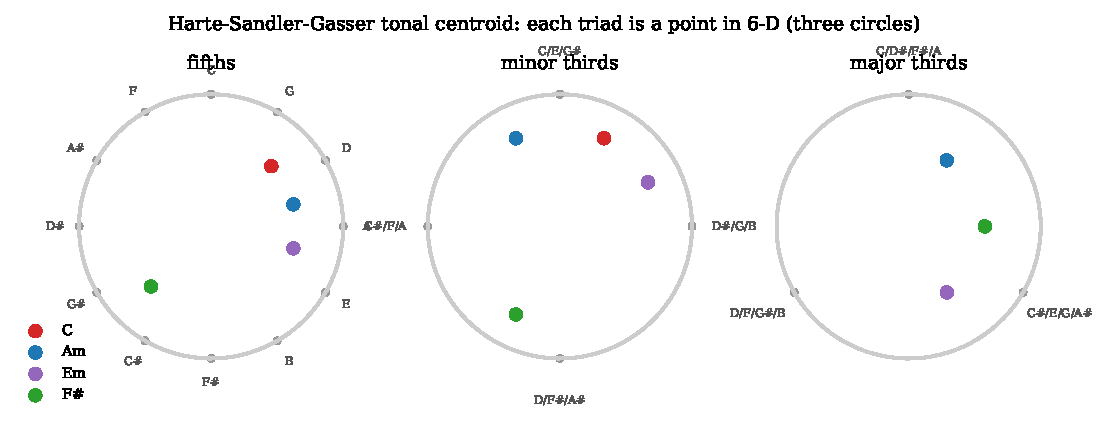
\includegraphics[width=0.92\linewidth]{figures/tonal_centroid.pdf}
\caption{Tonal centroids of four triads on the three circles. C and Am (an $R$ pair) are close on all three.}
\label{fig:centroid}
\end{figure}

\begin{notebookbox}
\sheet{07\_corpus\_analysis.ipynb} reruns \cref{tab:corpus} after \code{bash scripts/fetch\_data.sh};
\sheet{08\_audio\_centroid.ipynb} synthesises a progression, computes chroma, tonal centroid and HCDF, and compares
with librosa.
\end{notebookbox}

\begin{qa}
\Qu{Why reduce C7 to C before measuring Tonnetz distance?}
\A{The classical Tonnetz has only major and minor triads as faces; the reduction keeps the triad that carries the
chord's root and quality and discards the seventh.}
\Qu{What does the within-piece shuffle control for?}
\A{The chord vocabulary. A piece in one key uses nearby triads anyway; comparing with its own shuffles asks
whether the \emph{order} of chords is more local than the vocabulary alone implies.}
\Qu{Why is motion by a perfect fifth at distance 2 in $\Gamma$?}
\A{C$\xrightarrow{L}$Em$\xrightarrow{R}$G: the two triads share one note (G) and are linked through a triad that
shares two notes with each.}
\Qu{Name two reasons why pop corpora show more distance-4 transitions.}
\A{Stepwise root motion between major triads (IV--V, $\flat$VII--I) is idiomatic in rock and pop, and parallel
voice leading is common there; both are ``far'' in a common-tone metric.}
\Qu{How is the tonal centroid related to the Tonnetz?}
\A{It projects pitch classes onto circles of fifths, minor thirds and major thirds, the three lattice directions
of the Tonnetz, and averages over the chord's notes.}
\Qu{Suggest a way to test whether the Beethoven result is specific to Beethoven.}
\A{Run the same pipeline on the Distant Listening Corpus, which uses the same DCML format, grouped by composer and
era, and compare observed-minus-shuffled distances.}
\end{qa}
